\section{Constraining the Prevalence of High Energy GRBs using VLF measurements of the Ionosphere}

Similarly to GReX some preliminary work was carried out to use constrain the prevalence of Gamma Ray Bursts (GRBs) using a global Very Low Frequency (VLF) network to which there is a station in Birr. VLF monitoring is carried out using a global network of continuously operating transmitters and receivers. Each transmitter emits stable radio waves  (table \ref{tab:VLFstations}) from 15-30~kHz ranging from powers of kW to MW. These signals propagate throughout the ionosphere and VLF stations continuously record the amplitude and wave phase. As the waves are stable any variation can be attributed to the ionosphere and thus used as a tool to monitor fluctuations. By monitoring these signals continuously across many receiver paths high time resolution measurements of ionospheric disturbances produced by solar flares, lightning, energetic particle precipitation, and GRBs have been observed. 

GRBs are the most energetic explosions in the Universe (other than the Big Bang). They can last on timescales of a few milliseconds to hours and release in a few seconds more energy than the Sun will in its entire lifetime. They were first discovered in 1967 (\nref) by the \textit{Vela} military satellites.  There are two classes of progenitors that cause GRBs, collapsars which are associated with long GRBs and mergers which are associated with short GRBs.  Collapsars arise from the core-collapse of a massive star $(>8~\text{M}_\odot)$ and have known associations with broadlined Ic supernovae \citep{cotter_machine_2025}. Whereas, mergers manifest themselves in the form of merging compact binaries (\nref).

The brighest GRB ever observed occurred in October 2022 and was subsequently dubbed the Brightest of All Time (BOAT). GRB 2022109A (herein BOAT) was first detected by \textit{Fermi} and \textit{Swift} with an energy of $10^{54}~\rm erg$ with a redshift of $z=0.151$ and was confirmed across the entire electromagnetic spectrum.

\begin{table}[h]
\centering
\begin{tabular}{lcc}
\hline
\textbf{Station} & \textbf{Country} & \textbf{Frequency (kHz)} \\
\hline
DHO38 & Germany & 23.4 \\
GQD (Anthorn) & United Kingdom & 19.58 \\
NAA (Cutler) & United States & 24.0 \\
NLK & United States & 24.8 \\
NWC & Australia & 19.8 \\
VTX & India & 18.2 \\
JJI & Japan & 22.2 \\
\hline
\end{tabular}
\caption{Primary VLF transmitting stations used for ionospheric monitoring.}
\label{tab:VLFstations}
\end{table}

It has long been noted that exceptionally bright GRBs can cause ionospheric disturbances \citep{fishman_observation_1988} the BOAT is no exception. \citet{hayes_significant_2022} noted a significant disturbance noted at the VLF at the Rosse Observatory which is shown in the top panel in \cref{fig:BOATVLF}. As there is over a decade of stored data from VLF data from around the globe (\cref{fig:VLFlocations}) readily available it was hypothesised that the ionosphere analogous to GReX could be used as an all sky GRB monitor through monitoring the ionosphere. 

The BOAT was detected at $71^\circ$\textit{E}, $21^\circ$\textit{N}. The Rosse Observatory sits at  $7.9^\circ$\textit{W}, $53.1^\circ$\textit{N}. Using the haversine function, 

\begin{equation}
    d = 2r \arcsin\sqrt{\sin^2\left(\frac{\Delta \phi}{2}\right) + 
    \cos(\phi_1) \cdot \cos(\phi_2) \cdot 
    \sin^2\left(\frac{\Delta \lambda}{2}\right) }
\end{equation}

Using the above equation it's possible to calculate the great circle distance between approximate points in the ionosphere. The average Earth radius is, $6371 \rm ~km$ and it was in local afternoon (about 12:49 local solar time) in Birr when the VLF signal was detected. The signal would therefore have been probing the daytime D-region, with an effective reflection height of approximately $70~\rm km$,.  $\Delta\phi = 32.1^\circ$ and $\Delta \lambda = -78.9^\circ$ which gives the great circle distance of $\sim 7506$ km between the point above Earth where the BOAT was directly incident and Birr. \textit{Fermi} detected the BOAT at 13:16:59.000160, the VLF in Birr rises above the noise floor at 13:20:56 and peaks at 13:21:35. If it is assumed that the \textit{Fermi} detection and the time the gamma rays reach and illuminated atmosphere are simultaneously the apparent propagation velocity of the ionospheric response can be measured. If the velocity is measured at time of rise, $v_{\rm rise}$ is $31.7~\text{km}~\text{s}^{-1}$ and the velocity if measured at the time of the peak is $27.2~\text{km}~\text{s}^{-1}$. Seeing as there is a 39-second time differential between the rise and peak of the emission measured and relative velocities have been calculated the VLF perturbation may be represented using a simple ionisation–recombination response model \citep{hayes_solar_2021} in which the incident gamma-ray flux provides a time-dependent electron-production term. Although interpreting the delay as horizontal propagation gives apparent velocities, the available single-station observation cannot distinguish a travelling plasma disturbance from the delayed chemical and radiative response of the D-region.



\begin{figure}[h]
    \centering
    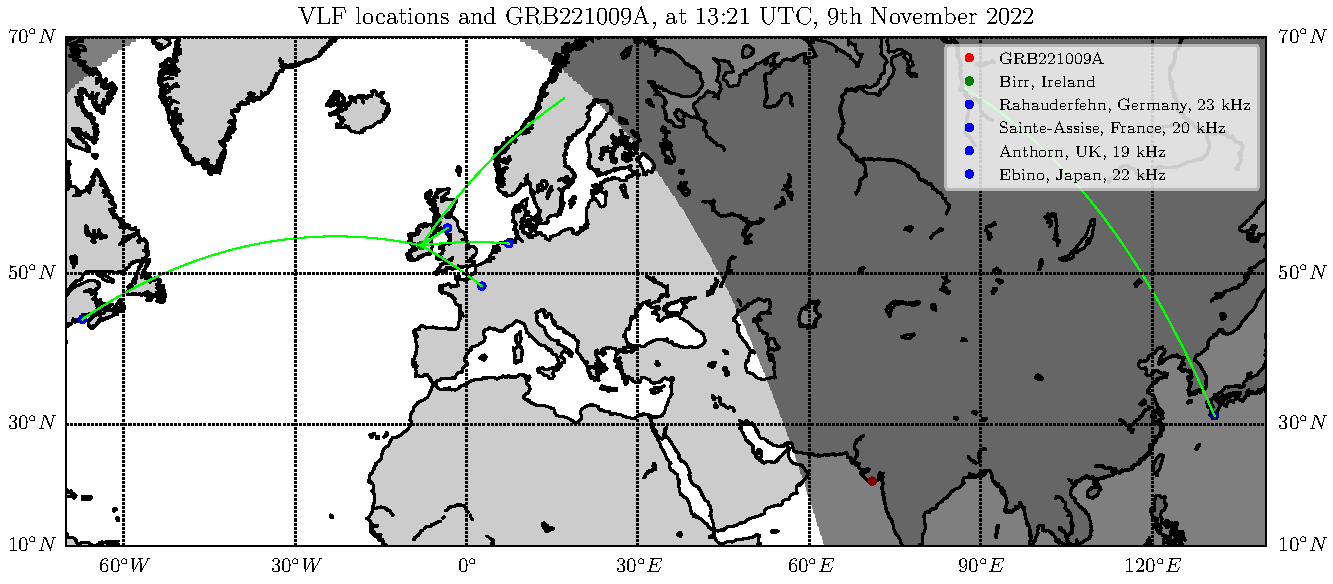
\includegraphics[width=\linewidth]{chapter8/plots/GRB221009A_VLF_locations.pdf}
    \caption{Mercator map with transmitting stations that were recorded on the day of the BOAT observation along with the incident area of the BOAT itself and the VLF recieving station in Birr.}
    \label{fig:VLFlocations}
\end{figure}

This disturbance prompted the exploration of the 4.63 years of VLF data collected in Birr. Developing a scraper too for both VLF archive\footnote{\url{https://vlf.ap.dias.ie/data/}} and  GRBWeb\footnote{\url{https://user-web.icecube.wisc.edu/~grbweb_public/}} to retrive the data it was then found that of the 8512 GRBs in the found in the GRBWeb catalogue 1039 occured during the period of data pulled from the archive (October 2020–March 2025) of those there were 364 data, shown in \cref{fig:fluencevstimeGRBs}.  


\begin{figure}[h]
    \centering
    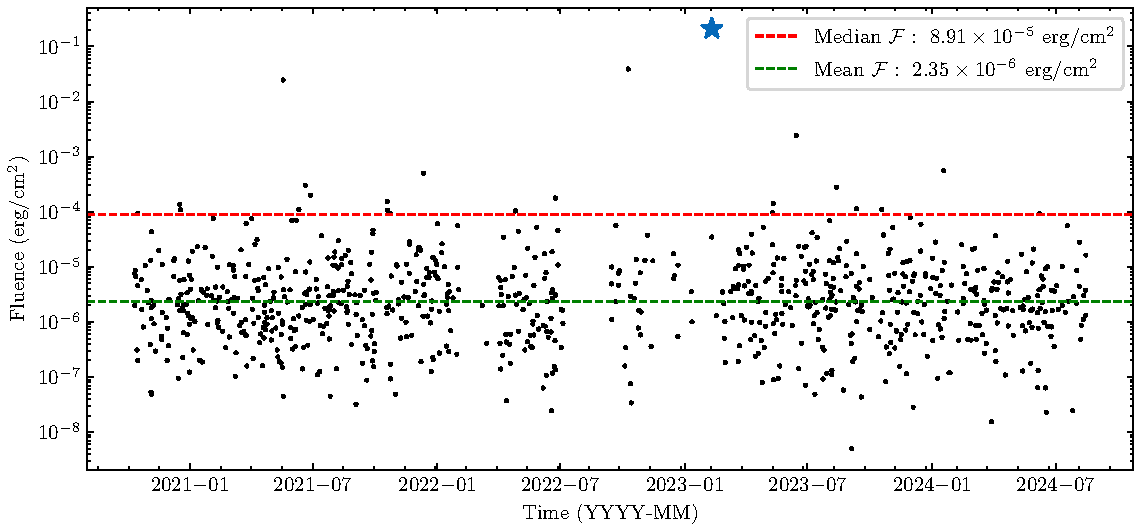
\includegraphics[width=0.9\linewidth]{chapter8/plots/fluence_vs_time.pdf}
    \caption{Fluence vs time of GRBs detected while VLF was operating. The dotted green line is the median, red is the mean and the BOAT are denoted by the blue star ($\star$). }
    \label{fig:fluencevstimeGRBs}
\end{figure}
 
For each of the GRBs the data was plotted $\pm30$ minutes to see if any other prominent ionospheric disturbances could be seen in addition to the BOAT as shown in \cref{fig:BOATVLF}. Each of the bursts were looked through by eye, but there was no clear ionospheric disturbances shown from the population of GRBs that were observed during VLF data recording. 

% \newpage
Similar to the GReX calculations from the previous sections constraints can be placed on the occurrence rate of high energy GRBs through VLF measurements. Taking the observing time as 4.63 years, the `on-time' as the fraction of observed GRBs\footnote{This assumes that \textit{Fermi}, ICECUBE and other similar observatories observe 100\% of GRBs.} to those detected (0.35) and the assumption that at some fluence GRBs will always disturb the ionosphere. This gives a 1.621 sky yrs. Using \cref{eq:k1_p} again, as its also one event the postier Gamma distribution is $\Gamma(2,\tau_1)$ where $\tau_1$ is the rate parameter which is equal to 1.621. The posterior peaks at an event rate of $0.62~\text{sky}^{-1}~\text{yr}^{-1}$ while the posterior mean is $1.23~\text{sky}^{-1}~\text{yr}^{-1}$. The corresponding 68\% and 95\% credible intervals are $0.44-2.03~\text{sky}^{-1}~\text{yr}^{-1}$ and $0.15-3.44~\text{sky}^{-1}~\text{yr}^{-1}$ respectively. As there is only one event detected, the posterior is quite broad. As VLF antennas are cheap to build and already have global infrastructure. One of the next steps forward in this programme would be to build a network of VLF receivers distributed across Ireland would provide multiple independent propagation paths through the ionosphere, enabling the spatial localisation of disturbances and with increased on sky time would further constrain ionospheric response to GRBs. 

\begin{figure}[h]
    \centering
    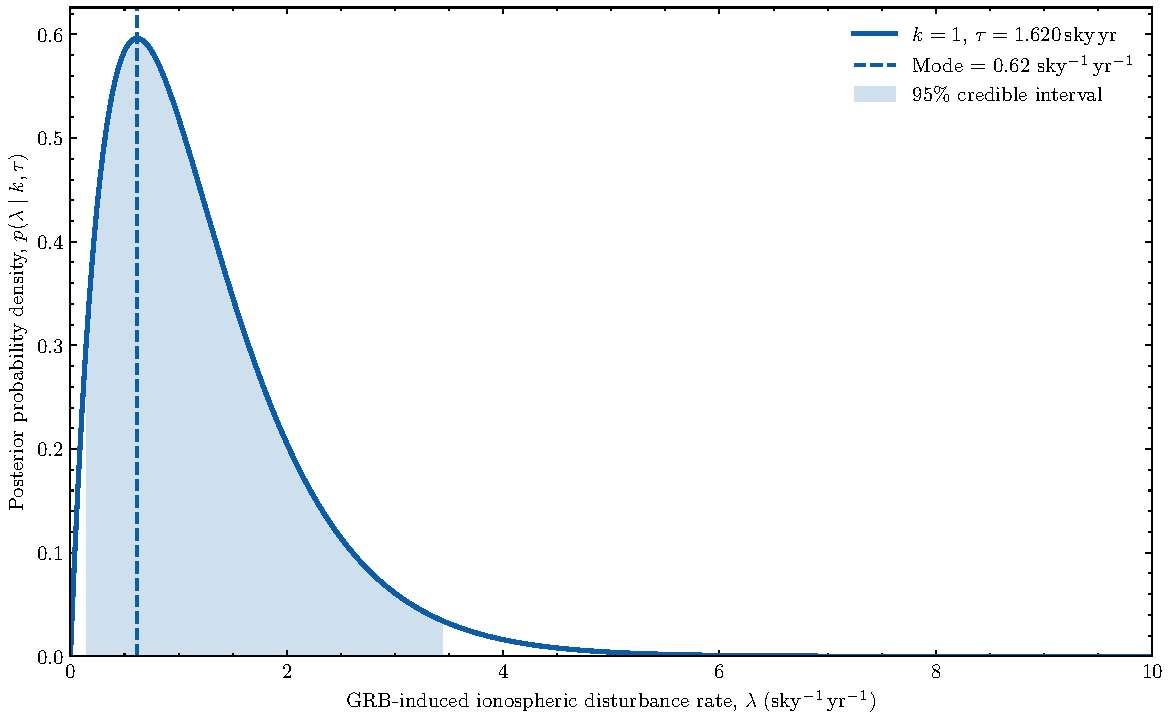
\includegraphics[width=0.9\linewidth]{chapter8/plots/GRB_ionosphere_poisson_posterior.pdf}
    \caption{Posterior distribution of GRB event rate $\lambda$ with shaded 95\% credible interval.}
    \label{fig:GRBposterior}
\end{figure}


\begin{figure}
    \centering
    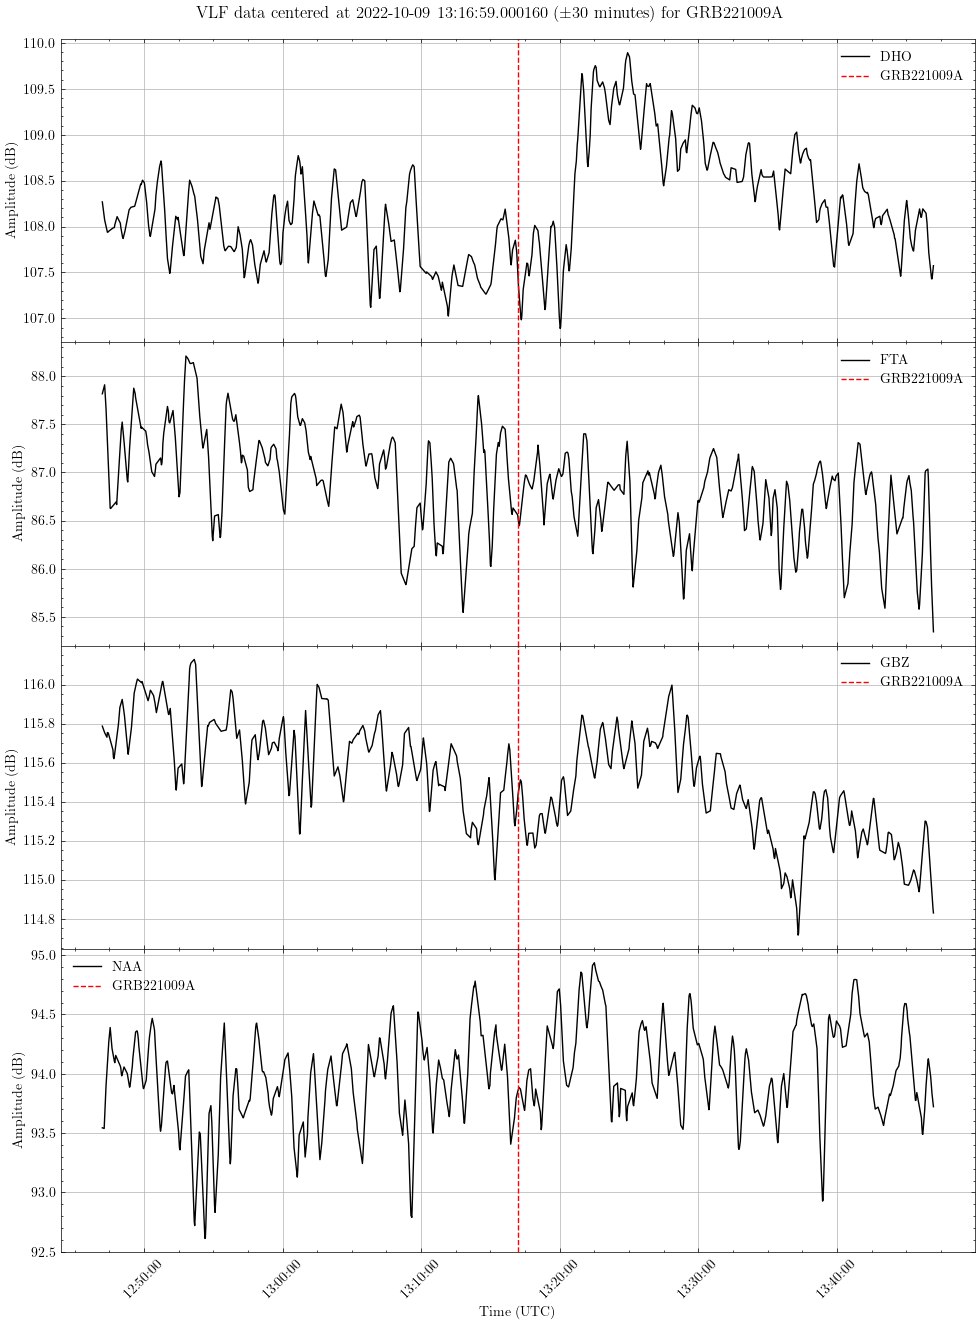
\includegraphics[width=\linewidth]{chapter8/plots/1GRB221009A.png}
    \caption{Example output from scraper scripts showing VLF data $\pm30$ minutes of a noted GRB emission. }
    \label{fig:BOATVLF}
\end{figure}


